% !TEX TS-program = pdflatex
% !TEX encoding = UTF-8 Unicode

\documentclass[12pt]{article}
%\documentclass[10pt,twocolumn]{article}

\usepackage[utf8]{inputenc} % set input encoding (not needed with XeLaTeX)

%%% PACKAGES
\usepackage{amsmath}
\usepackage{amsfonts}
\usepackage{graphicx}
\usepackage{booktabs}	 % for much better looking tables
\usepackage{array}	 % for better arrays (eg matrices) in maths
\usepackage{breqn} 	% breaks lines
\usepackage{authblk}	% helps with authors on title page
\usepackage{multirow}
\usepackage{fancyhdr}

\pagestyle{fancy}

\lhead{}
\chead{DRAFT --- NOT FOR PUBLIC RELEASE}
\rhead{}


%----------------------------------------------------------------------------
\begin{document}
\pagenumbering{gobble}
%----------------------------------------------------------------------------
\renewcommand\Authfont{\small}
\renewcommand\Affilfont{\itshape\footnotesize}
%----------------------------------------------------------------------------
\title{
	{Educational Scheduling as a Mixed Integer Programming Model}\\
	\vspace{2cm}
	{\large Final Paper for ETM 540 (Fall 2016)}\\
	{\large Taught by Professor Tim Anderson}\\
	\vspace{2cm}
}

% \title{Educational Scheduling as a Mixed Integer Programming Model}


%----------------------------------------------------------------------------
\author[1,2]{Will Kearney}
\author[1,2]{Sonimar Poppe}
\author[2]{Niguel Morfin}
\author[2]{Asrar Ahmed Syed}
\affil[1]{Portland Public Schools}
\affil[2]{Engineering and Technology Management, Portland State University}
%----------------------------------------------------------------------------
%\date{} % Activate to display a given date or no date (if empty),
         % otherwise the current date is printed 
%----------------------------------------------------------------------------

\maketitle
\newpage

\begin{abstract}
This paper demonstrates that Mixed Integer Programming (MIP) is an effective method to schedule middle school courses. We provide a background on the difficulties scheduling courses, why this is important, et cetera...
\end{abstract}

\newpage

\tableofcontents
\newpage

\pagenumbering{arabic}

\section{Introduction}

Coming soon...

\section{Problem Statement}

In 2007 the governor signed House Bill 3141 into law, requiring that K-5 students receive physical education of 150 minutes per week and 6-8 students receive 225 minutes per week.  For students in grades K-5, this translates to 30 minutes daily; for students in grades 6-8, this translates to 45 minutes daily. Every school district is to be in compliance by the 2017-18 school year. No additional funding will be provided by the state to help school districts make this changes.

Portland Public Schools (PPS) is currently evaluating the best way to comply with the new physical education requirements for students in grade 6-8 in a cost effective way, while simultaneously ensuring students remain in their core classes and are able to continue taking their desired electives. PPS is increasing the amount of periods it offers in middle school from 6 to 7 by reducing each period from 1 hour to 45 minutes.  The school district would like to optimize the current student’s schedules and add physical education for all the students

For the new schedule all students and full time teachers must have a lunch break either in Period 4 or Period 5. In addition full time teachers must have a planning period in which they are not assigned to any class. Students must also take the necessary core classes for their grades and teachers must not teach a class they are not currently teaching. Each class must not be bigger than the maximum allowed size for the particular course.

PPS is also curious to see if the new way to schedule classes will result in better class sizes.

PPS identified one middle school to use during our test case.  The data was extracted from the district's Student Information System (SIS) database and anonymized to protect the privacy of each student and teacher.

\section{Our Approach}

Coming soon...

\section{Data}

Coming soon...


\section{Model Formulation}

\begin{table}[]
\centering
\caption{The data notation used in our formulation}
\label{tab:data-notation}
\begin{tabular}{ll}
\hline
$maxClassSize_{c}$ & Maximum number of students \\
 & permitted in class $c$ \\
$maxNumPeriods_{t}$ & Maximum periods teacher $t$ can teach\\
$enrolled_{s,c}$ & If student $s$ is currently taking course $c$\\
$core_{c}$ & Indicator is course $c$ is a core course \\
\hline
\end{tabular}
\end{table}


\begin{table}[]
\centering
\caption{The index notation used in our formulation}
\label{tab:index-notation}
\begin{tabular}{ll}
\hline
$s$ & $\in$ Set of students \\
$t$ & $\in$ Set of teachers \\
$c$ & $\in$ Set of courses \\
$p$ & $\in$ Set of periods \\
\hline
\end{tabular}
\end{table}


\subsection{Decision Variables}

% student decision variables
\begin{equation}
	X_{s,c,p} = 
	\begin{cases}
		1, & \text{if student}\ s \text{ is assigned to course}\ c \text{ in period}\ p	\\
		0, & \text{otherwise}
	\end{cases}
\end{equation}

and

% staff decision variables
\begin{equation}
	Y_{t,c,p} = 
	\begin{cases}
		1, & \text{if teacher}\ t \text{ is assigned to course}\ c \text{ in period}\ p	\\
		0, & \text{otherwise}
	\end{cases}
\end{equation}

\subsection{General Constraints}

The first constraint set is general in that it guarantees some basic conditions regardless of any other criteria that may be additionally required; it is the ``base model'', so to speak.

\begin{equation} \label{eq:every-student-fully-scheduled}
	\displaystyle \sum_{c} X_{s,c,p} = 1 \quad \forall s,p
\end{equation}

\begin{equation} \label{eq:double-book-teachers}
	\displaystyle \sum_{c} Y_{t,c,p} \leq 1 \quad \forall t,p
\end{equation}

Constrainst~\ref{eq:every-student-fully-scheduled} ensures that every student is full scheduled (i.e. taking exactly one course every period of the day). Similarly, constrainst~\ref{eq:double-book-teachers} ensures that no teachers are double-booked; in other words, each teacher can be assigned to at maximum one course during each period.

\begin{equation} \label{eq:only-one-class}
	\displaystyle \sum_{p} X_{s,c,p} \leq 1 \quad \forall s,c
\end{equation}

Constraint~\ref{eq:only-one-class} guarantees that a student can't take a given class more than once per day.

\begin{equation} \label{eq:lunch-constraint}
\begin{split}
	X_{s,lunch,3} + X_{s,lunch,4} = 1 \quad \forall s \\
	Y_{t,lunch,3} + Y_{t,lunch,4} = 1 \quad \forall t
\end{split}
\end{equation}

Every student and teacher should be scheduled to lunch in one of two lunch periods. In a 7 period day, lunch periods are 3 and 4; in an 8 period day, lunch periods are 4 and 5. Constraint~\ref{eq:lunch-constraint} illustrates a 7 period day.


\subsection{Capacity}

Most obviously, capacity can be thought of in terms of the number of students assigned to a particular class and period. The maximum number of students allows in a class is denoted by $maxClassSize_{c}$, which has an upper bound of 30, though it is often lower. Class size capacity is enforced as follows:

\begin{equation} \label{eq:class-size-capacity}
	\displaystyle \sum_{s} X_{s,c,p} \leq maxClassSize_{c} \cdot \displaystyle \sum_{t} Y_{t,c,p} \quad \forall c,p
\end{equation}

Constraint~\ref{eq:class-size-capacity} restricts the maximum number of students assigned to a class and period to the maximum number of seats available. It is important to recognize that multiple sections of a course can be taught during the same period, which is why equation~\ref{eq:class-size-capacity} includes the decision variable $Y_{t,c,p}$. Because the maximum class size is multiplied by the number of teachers assigned to that course and period, an arbitrary number of teachers can be assigned to help reduce class size by increasing the number of sections (subject to teacher availability constraints, of course).

Capacity can also be thought of in terms of the numbers of courses each teacher can be assigned. Largely, this is dictated by financial constraints. Teachers workloads are permitted on the basis of full-time equivelent (FTE) units; an FTE of 1 is equivalent to a full-time teacher. Additionally, full-time teachers are required to have at least one planning period per day.

\begin{table}[]
\centering
\caption{The maximum number of periods a teacher is allowed to teach, based on their FTE workload and the number of periods in the day. For example, in a 7 period schedule, a teacher with FTE 0.75 can teach a maximum of 5 periods.}
\label{tab:max-num-periods}
\begin{tabular}{lcccc}
             & \multicolumn{4}{c}{FTE} \\ \cline{2-5} 
             & 0.25 & 0.5 & 0.75 & 1.0 \\ \cline{2-5} 
7 period day & 1    & 3   & 5    & 6   \\
8 period day & 2    & 4   & 6    & 7  
\end{tabular}
\end{table}

Thus, a full-time teacher can teach a maximum of periods equal to the total number of periods minus one. Part-time teachers (defined as less then 1 FTE) can teach a maximum of periods equal to the total number of periods multiplied by their FTE amount, rounded down to the nearest whole number. Part-time teachers are not explicitely allocated a planning period, because they already have unscheduled periods due to their FTE limitation. Table~\ref{tab:max-num-periods} shows the maximum number of periods teacher of various FTE workloads are permitted to teach for a 7 period and 8 period schedule.

\begin{equation} \label{eq:number-courses-taught}
\begin{split}
	\displaystyle \sum_{c,p} Y_{t,c,p} \geq 1 \quad \forall t \\
	\displaystyle \sum_{c,p} Y_{t,c,p} \leq maxNumPeriods_{t} \quad \forall t
\end{split}
\end{equation}

Constraint~\ref{eq:number-courses-taught} ensures that no teacher is scheduled to more than their maximum number of periods; additionally, each teacher must teach at least one period.


\subsection{Specific Course Requirement}

In our model, we wanted every student to be assigned to the same core classes they are currently taking, denoted by the set $coreEnrolled_{s}$. This requirement was formulated as follows:

\begin{equation} \label{eq:required-core}
	\displaystyle \sum_{p} X_{s,c,p} \geq enrolled_{s,c} \cdot core_{c} \quad \forall s,c
\end{equation}

Thus, if a student is enrolled in a course ($enrolled_{s,c} = 1$) and the course is a core course ($core_{c}= 1$), the student must be assigned to the course in one period.

\subsection{Consecutive Period Assignment}

Ideally, part-time teachers would be scheduled only in consecutive periods. To model this, we invoked a formulation used for spatial contiguity based on a theory of network flows in a connected graph \cite{shirabe}.

A 7-period day can be thought of as a connected graph of 7 nodes, where each node (representing a period) is connected to its adjacent nodes (representing consecutive periods). Each node can either be scheduled or not; the set of scheduled nodes forms a sub-graph. We seek a solution in which this sub-graph is connected, or at least one path exists between each pair of nodes in the subgraph. This is equivelent to saying a path must exist between each scheduled node and a particular scheduled node. Path finding between every scheduled node and one specific scheduled node in a connected set is analogous to fluid movement from multiple sources to a single sink in a connected network.

First, binary indicator variables are created that are activated when a teacher is scheduled during a particular period.

\begin{equation}
	S_{t,p} = 
	\begin{cases}
		1, & \text{if teacher}\ t \text{ is scheduled in period}\ p \\
		0, & \text{otherwise}
	\end{cases}
\end{equation}

\begin{equation} \label{eq:link-teacher-period-indicator}
	S_{t,p} = \displaystyle \sum_{c} Y_{s,c,p} \quad \forall t,p
\end{equation}

Equation~\ref{eq:link-teacher-period-indicator} links the indicator variable to the teacher decision variable. Variables are created to indicate sinks and measure flow as follows:

% sink
\begin{equation}
	w_{t,p} = 
	\begin{cases}
		1, & \text{if node/period}\ p \text{ is a sink for teacher}\ t \\
		0, & \text{otherwise} 
	\end{cases}
\end{equation}

% amount of flow
\begin{equation}
	flow_{t,p,q} \in \mathbb{Z}
\end{equation}

where $flow_{t,p,q}$ is a continuous variable measuring the amount of flow from node $p$ to node $q$ in the set of nodes (periods) for teacher $t$.

The following constraint set guarantees to select consecutive region from a set of nodes regardless of other constraints imposed. It is expressed as a set of linear equations:

% Ensures net flow moves towards sink; avoids cycles in graphs
\begin{equation} \label{eq:net_flow}
\begin{split}
	\displaystyle\sum_{q|(p,q) \in A} flow_{t,p,q} - \displaystyle\sum_{q|(q,p) \in A} flow_{t,p,q} \geq
	 S_{t,p} - M \cdot w_{t,p}
	\quad \forall t,p
\end{split}
\end{equation}

% Ensures there is no flow in or out of the subgraph
\begin{equation} \label{eq:flow_out_of_subgraph}
	\displaystyle\sum_{q|(p,q) \in A} flow_{t,p,q} \leq (M-1) \cdot S_{t,p} \quad \forall t,p
\end{equation}

% Ensure if a sink is activated, it is also activated as a period in the subgraph
\begin{equation} \label{eq:if-sink-then-period}
	S_{t,p} \geq w_{t,p} \quad \forall t,p
\end{equation}

% Make sure there is one 'sink' per teacher
\begin{equation} \label{eq:one-sink}
	\displaystyle\sum_{p} w_{t,p} = 1 \quad \forall t
\end{equation}

where $M$ is a non-negative integer indicating the maximum allowable number of periods to be scheduled for a teacher and $A_{p,q}$ is the set of adjacent nodes or periods.

In general, constraint~\ref{eq:net_flow} ensures net flow moves towards a sink and avoids cycles in graphs, constraint~\ref{eq:flow_out_of_subgraph} ensures there is no flow in or out of the subgraph (i.e. set of scheduled periods), constraint~\ref{eq:if-sink-then-period} ensures that if a period is chosen as the sink it also must be scheduled, and constraint~\ref{eq:one-sink} ensures that there is exactly one sink per teacher schedule. The reader is deferred to \cite{shirabe} for a more detailed explanation.

\begin{figure}
	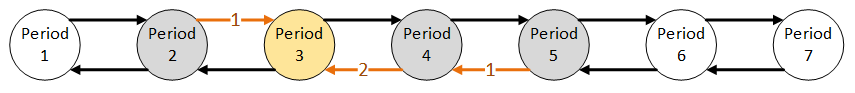
\includegraphics[width=\linewidth]{./flow_diagram}
	\caption{A flow diagram of a 7 period day for a particular teacher. The grey and yellow nodes represent periods in which the teacher is scheduled; the yellow node represents the sink. Black arrows are possible flow avenues between adjacent nodes; those that are experiencing flow are labelled with their flow value. For example, period five contributes a flow of 1 to period four, which therefore contributes a total of 2 (1 from period five, plus an additional 1), which drains into the sink located at period three.}
	\label{fig:flow-diagram}
\end{figure}

\section{Objectives}

\subsection{Electives}

This objective seeks to maximise the number of students assigned to the same electives they are currently taking. This is accomplished by creating a new variable

\begin{equation}
	numCurrentElectives_{s} \in \mathbb{Z}
\end{equation}

that counts the number of electives a student is assigned to that they are currently taking. This variable is linked as follows:

\begin{equation} \label{eq:link-num-electives}
	numCurrentElectives_{s} = \displaystyle\sum_{c,p} X_{s,c,p} \cdot (1-core_{c}) \cdot enrolled_{s,c} \quad \forall s
\end{equation}

By maximizing $numCurrentElectives_{s}$, we maximize the number of electives students are taking in the model solution that they are currently taking. Of course, this could be easily modified to maximize for elective preference as well (i.e. we are essentially using what students are currently taking as a proxy for how they might rank their desired electives; although this might be in reality a bad assumption, is is convenient from a data-gathering and modeling perspective).


\section{Results}

\subsection{Model Results}

\begin{figure}
\centering
	% [width=8cm] 
	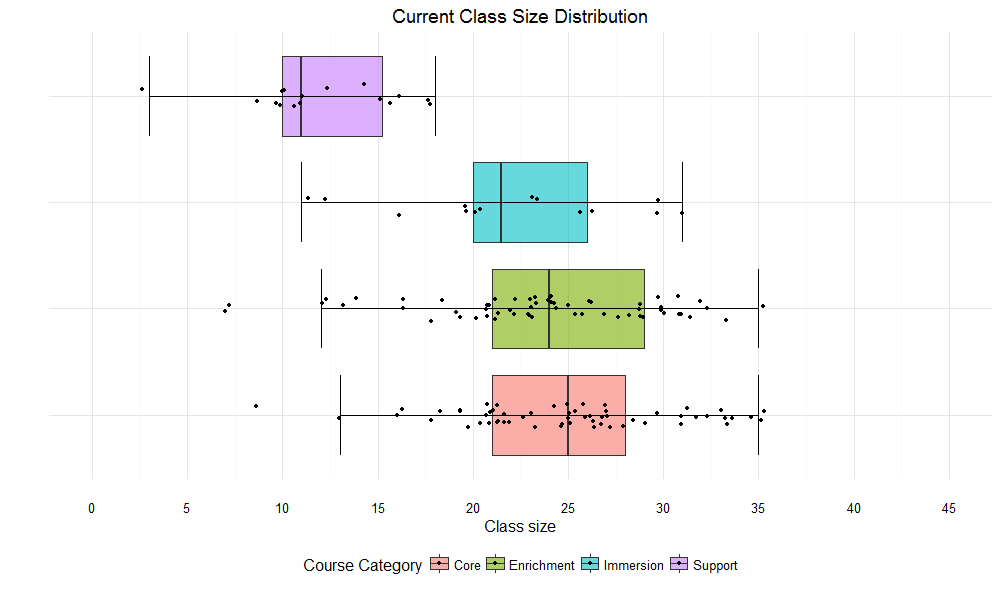
\includegraphics[width=\linewidth]{./current_class_size_distribution}
	\caption{The current class size distribution. There are some classes above 30 students, something parents expressed concern over in various community meetings.}
	\label{fig:current-class-size-distribution}
\end{figure}

\begin{figure}
\centering
	% [width=8cm] 
	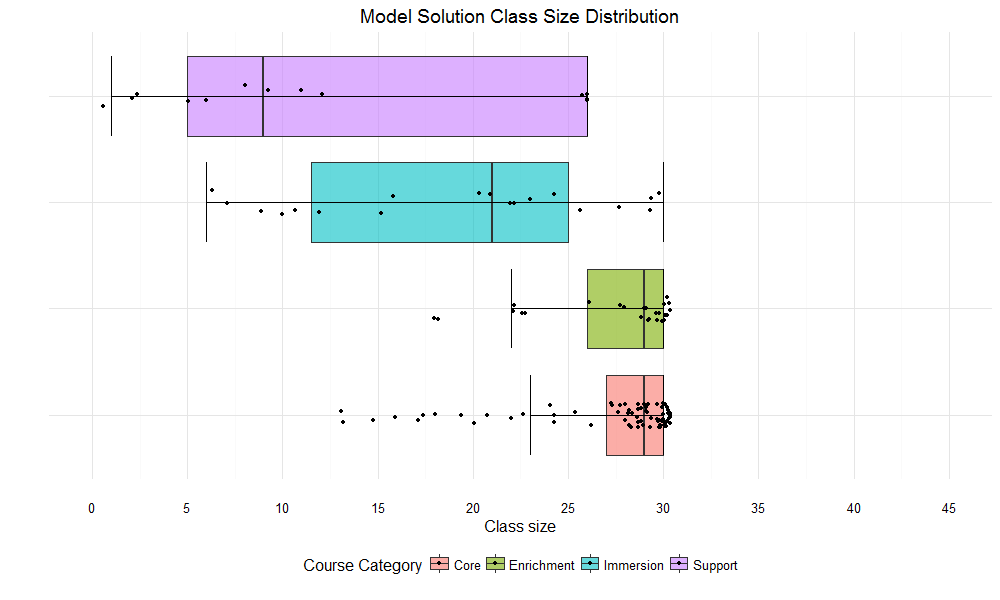
\includegraphics[width=\linewidth]{./model_solution_class_size_distribution}
	\caption{The class size distribution produced by the optimization model. There are no longer any classes above 30 students.}
	\label{fig:model-class-size-distribution}
\end{figure}

As can be seen by comparing figure~\ref{fig:current-class-size-distribution} and figure~\ref{fig:model-class-size-distribution}, the optimization model produces a solution in which no classes are enrolled with more than 30 students. However, this comes at a trade-off; table~\ref{tab:num-electives-lost} shows the number of students who are no longer able to take electives they are currently enrolled in. 208 students are taking all their current electives; 308 students are no longer taking one of their current electives; and 22 students are no longer taking two of their current electives.

\begin{table}[]
\centering
\caption{The number of students who are no longer taking electives they are currently enrolled in. 208 students are taking all their current electives; 308 students are no longer taking one of their current electives; and 22 students are no longer taking two of their current electives.}
\label{tab:num-electives-lost}
\begin{tabular}{ll}
\hline
Current Electives Lost & Number of Students \\ \hline
0                      & 208                \\
1                      & 308                \\
2                      & 22                 \\ \hline
\end{tabular}
\end{table}

This intuitively makes sense; as we decrease the maximum allowed class size, fewer students are able to take popular electives and must be displaced. One solution might be to hire more teachers for a desireable elective, or increase specific class sizes based on demand and expected educational impact.

\subsection{Model Tractability}

The initial model (i.e. solving without the PE requirement) had a total of 108846 rows and 200519 columns. 199939 of the variables were binary. The Gurobi solver had difficulty finding initial feasible integer solutions without the use of heuristics. Ultimately, we virtually always used the ``feasibility pump'' \cite{Fischetti2005} heuristic in order to find an initial feasible integer solution.

The model was run on an Intel Xeon E3-1240 CPU using all 8 threads. The model reached 0.19\% of proven optimality within 47 minutes; an additional 70 minutes of runtime failed to improve the incumbent solution.


\section{Future Work}

Coming soon...

\section*{Acknowledgement}

We'd like to thank Shawn Helm at Portland Public Schools for his general guidance and savvy model-building and Dr. Tim Anderson at Portland State University for teaching us his ways and assisting us in model formulation.

\bibliography{./education-scheduling-mip-model-paper}
\bibliographystyle{plain}

\end{document}






